\documentclass[UTF8]{ctexart}

\usepackage{subfiles}  

%下面的语句, 引入你的头部设置文件
\usepackage{C:/phpStorm_proj/02_myself_ID_EGO/+100_latex_all_math_sel/myPreamble} 
%必须是绝对路径,才能让各个tex在单独编译时使用到

\title{物理}


%---------------------------------


\begin{document}
	\tableofcontents % 生成目录
	\date{} % 若不写这句, 则默认也会渲染出日期, 所以我们要手动赋空值
	\maketitle  %这行代码, 让你前面的 title, author, date生效
	
	
	\section{摆的等时性}
	
	摆的等时性 : 无论摆动的幅度大还是小, 完成一次摆动的时间是一样的.	
	
	各种机械摆钟, 就是根据这个原理制作的.
	
	摆绳越长, 往复摆动一次的时间(即周期), 也就越长.
	
	
~\\
\hrule
~\\
	
	
	
	\section{质量 mass}
	
	\textbf{质量: 物体所含物质的多少, 叫做``质量" mass.} 公式中就用其首字母 m 来表示. \\
	
	质量的单位是:	 \\
	- 1 t 吨 = 1000 kg \\
	- 1 kg 千克(即公斤) \\
	- 1 g 克 = 1000 mg \\
	- 1 mg 毫克 \\
	
	地球的质量 = $ 5.97237 \cdot 10^{24} \ kg $ \\
	太阳的质量 = $ 1.9891 \cdot 10^{30} \ kg $ \\
	
	称质量的工具: 秤  \\
	
	\textbf{质量无关``物态": 一块冰融化成水, 其质量不会改变.} \\	
	质量也无关``所处的位置": 一个东西在地球上, 或带到太空里, 其质量不会改变. \\
	即: 物体的质量, 不随它的物态, 位置而改变. 
	
	
	~\\
	\hrule
	~\\
	
	
	\section{$\text{密度}\rho =\frac{\text{质量}m}{\text{体积}V}$}
	
	同一种物体, 体积越大, 质量越大. \\
	密度 density : 由某种物质组成的物体的``质量", 与它``体积"之比, 就是这种物体的``密度". 
	
	\begin{align*}
		\boxed{
			\text{密度}\rho =\dfrac{\text{质量}m}{\text{体积}V}
		}
	\end{align*}

	这个公式就是说: \textbf{``密度"在数值上, 等于``物体单位体积的质量".} \\

	密度ρ的单位, 是由``质量的单位" 和 ``体积的单位" 共同组成的. 即, \textbf{密度的基本单位就是: $ kg/m^3$ (千克/立方米), 或 $ g/cm^3$ (克/立方厘米).} \\

	这两个密度单位的关系是: 
	\begin{align*}
		\boxed{			
		1 g / cm^3 = 1 \cdot 10^3 kg/m^3
		}
	\end{align*}
	1 克/立方厘米(克每立方厘米) = 1000 千克/立方米(千克每立方米) \\
	
	
	
	~\\
	\hrule
	~\\
	
	
	
	\section{大气压强}
	
	\subsection{标准大气压强 :  $1.013\cdot 10^5\ P_a$}
	
	大气压强, 简称为大气压(atmosphere), 或气压。\textbf{注意:大气压是"大气压强"的简称,不是"大气压力"的简称.} \\
	
	大气压产生的原因: 由于大气受到重力的作用而产生. \\
	大气压的方向: 同液体一样, 大气朝向各个方向都有压强的. \\
	
	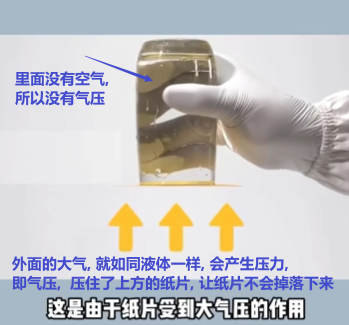
\includegraphics[width=0.3\textwidth]{img/0024.png}
	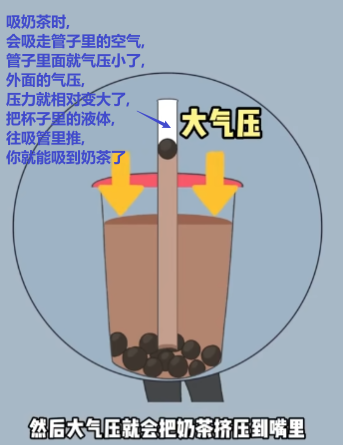
\includegraphics[width=0.3\textwidth]{img/0025.png}
	
	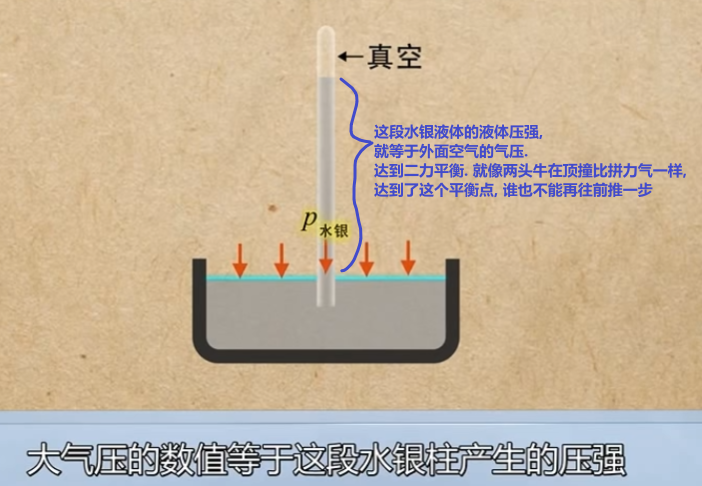
\includegraphics[width=0.3\textwidth]{img/0026.png}	
	
\includegraphics[width=0.3\textwidth]{img/0028.png}
	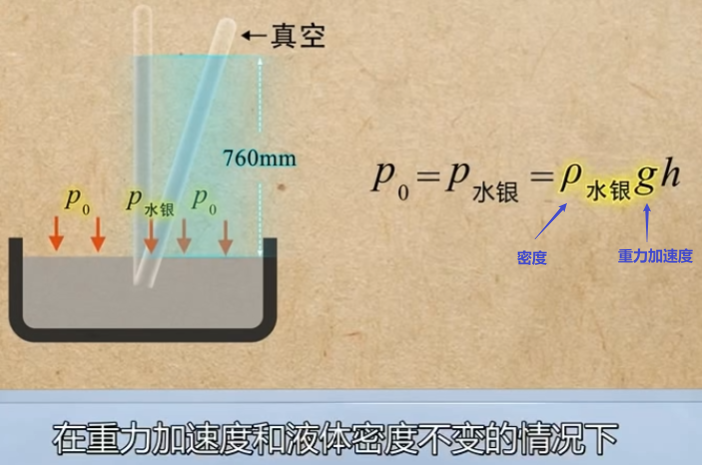
\includegraphics[width=0.3\textwidth]{img/0029.png} \\
	
	水银柱产生的压强 $p_{\text{水银}}=\text{标准大气压}p_0$, 根据压强公式 p=ρgh, 在水银密度ρ不变, 重力加速度g=9.8N/kg, 标准大气压 $p_0$,  这三个变量都不变的情况下, 显然水银柱的高度h 就不会改变.
	
	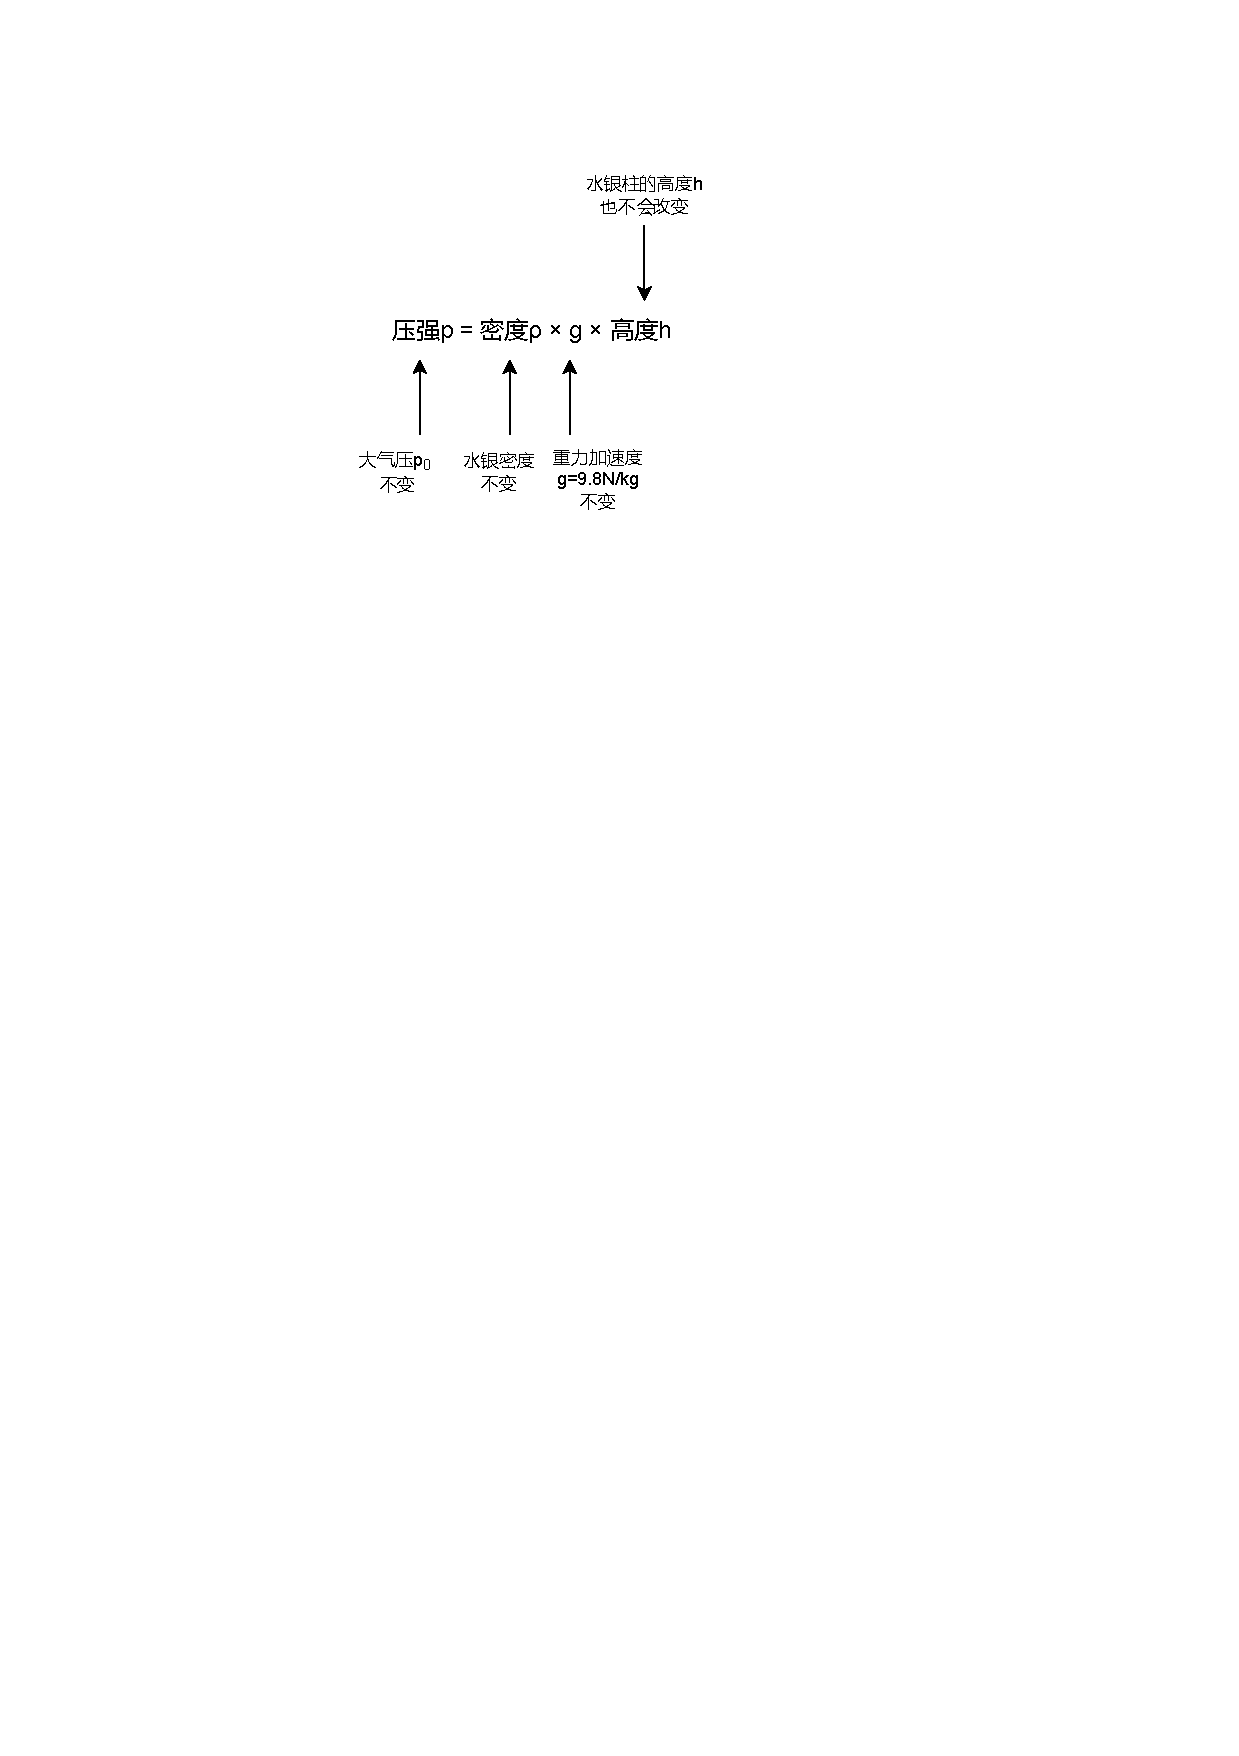
\includegraphics[width=0.3\textwidth]{img/0031.pdf} 
	
	同时这也说明, 某液体或气体深处的压力的大小, 跟其质量m的多少无关. 即使水银柱倾斜过来, 水银柱中水银的体积增加, 质量m增加, 它的压强p也不会改变. \\
	
	注意:只有在水银柱上部的空间是``真空"时, 水银柱的压强才跟大气压强相等. 如果水银柱上方不是真空, 而是混有空气, 则这段空间的气体, 也会对水银柱产生压强. 在这种情况下, 就是这个压强与水银柱产生的压强之和, 才等于大气压强.
	
	即: 管内水银柱的高度, 只随外界大气压的变化而变化, 而和管子的粗细、倾斜角度、管的长度, 及将玻璃管提起还是下压等因素无关. 只与水银柱的竖直高度有关. \\
	
	注意: 大气的密度是变化的, 在地面附近, 空气的密度较大, 随高度的增加, 空气的密度越来越小. \\
	
	所以, \textbf{在地表的大气压下, 压得水银柱高度为760 mm. 反过来说, 我们就把这样大小的大气压, 叫做``标准大气压" $p_0$.}
	
	\begin{align*}
		\boxed{
			\underset{\text{标准大气压}}{\underbrace{p_0}}=\underset{\text{水银密度}13.59g/cm³}{\underbrace{\rho }}\cdot \underset{9.8N/kg}{\underbrace{g}}\cdot \underset{0.76m}{\underbrace{h}}=1.013\cdot 10^5\ P_a			
		}
	\end{align*}
	
	水银的密度, 是水的密度的13.6倍. 
	
	\textbf{在粗略计算中, 标准大气压可以取为 $1×10^5 Pa$.}
		
	\vspace{1em} 
	
	
	
	\subsection{``标准大气压"下的水柱的高度是 10.336米}
	
	如果玻璃管中装的是水呢?	
	\begin{align*}  % 支持每行编号. 若不需要编号, 就用 align*环境
	& \underset{\text{标准大气压}}{\underbrace{p_0}}=p_{\text{水银}}=p_{\text{水}}\\
	& \text{即:\ }\underset{\text{水银密度}13.59g/cm³}{\underbrace{\rho }}\cdot \underset{9.8N/kg}{\underbrace{g}}\cdot \underset{0.76m}{\underbrace{h}}=\underset{\text{水的密度1.0\ }kg/m³}{\underbrace{\rho }}\cdot \underset{9.8N/kg}{\underbrace{g}}\cdot \underset{\text{水柱的高度}}{\underbrace{h}}\\
	& \text{最终会得到\ }h_{\text{水}}=10.336m\\ 
	\end{align*}
		
	\vspace{1em} 
	
	
	
	\subsection{(1)高度越高, 空气密度越小, 气压就越低. (2)气压越低, 沸点也就越低}
	
	从气压公式也可知道: \textbf{随着高度的升高(即 深度h 的减少. 你只需把空气想象成大海, 越接近地表的空气, 就如同海底的深度一样, 深度最大. 即 h最大. 这样, 随着海拔的增加, 越往天上去, 空气的深度h就越小, 气压就越小).}  换种说法就是: 海拔升高,空气就越稀薄,密度越小,所以大气压会减小. 瓶中的空气的气压值超过了外面的气压, 就会将瓶中的水挤压到玻璃管中,  水柱的高度就会逐渐升高。
	
	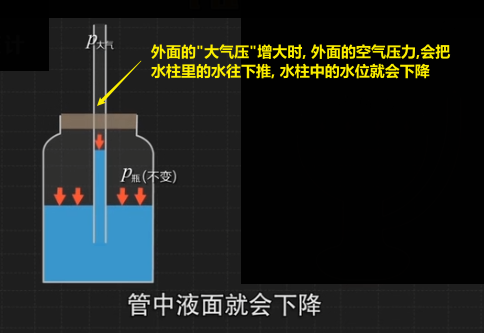
\includegraphics[width=0.45\textwidth]{img/0032.png} 
	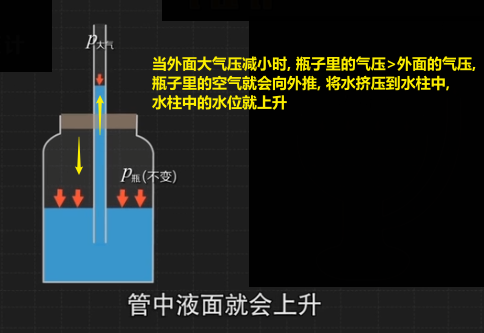
\includegraphics[width=0.45\textwidth]{img/0033.png} 
	
	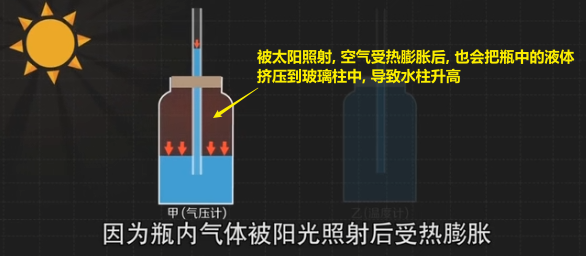
\includegraphics[width=0.45\textwidth]{img/0036.png} 	
	
	在海拔3000m 以内, 大约每升高10m, 大气压减小100 Pa. \\
	
	液体的沸点跟外部压强有关。当液体所受的压强(比如气压)增大时, 沸点也升高; 压强减小时,沸点也降低.   \\	
	- 蒸汽锅炉里的蒸汽压强,约有几十个大气压,锅炉里的水的沸点可在200℃以上. \\	
	- 在高山上煮饭,比如青藏高原, 水的沸点仅为 84-87℃, 水就沸腾了,但饭不易熟. 所以必须使用压力锅做饭, 以增强压力, 让沸点升高.
	
	
	
	
	
	
	
	\vspace{1em} 
	
	\subsection{自制气压计: 瓶中必须存在空气, 才能有气压, 才能在瓶中内外造成气压差.}
	
	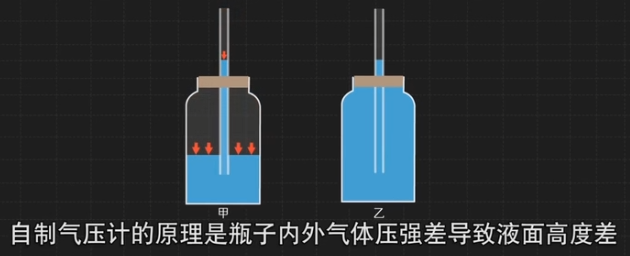
\includegraphics[width=0.45\textwidth]{img/0034.png} 
	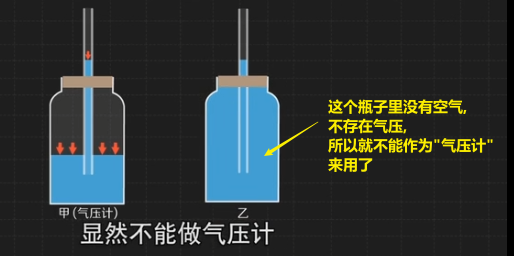
\includegraphics[width=0.45\textwidth]{img/0035.png} 
		
	
	~\\
	\hrule
	~\\
	
	
	\subsection{流体压强 : 流速越大的位置, 压强越小}
	
	\begin{tcolorbox}[title = {例},boxrule={0.1em},colframe={black!10}, colback={black!3},colbacktitle={black!10},coltitle={black}]
	两张垂落的纸, 向中间吹气, 纸张不会向外扬起, 而是向内靠拢. \\

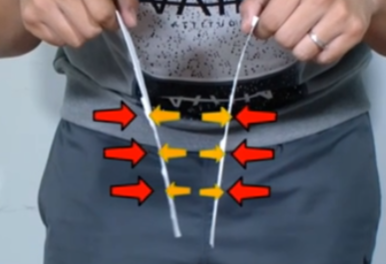
\includegraphics[width=0.45\textwidth]{img/0037.png}
	\end{tcolorbox}

	
	\begin{tcolorbox}[title = {例},boxrule={0.1em},colframe={black!10}, colback={black!3},colbacktitle={black!10},coltitle={black}]
	用纸做一个桥, 向桥洞里吹气, 桥会塌掉. \\


\includegraphics[width=0.45\textwidth]{img/0038.png} 	
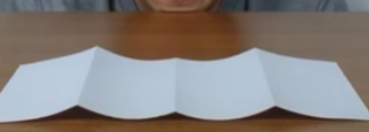
\includegraphics[width=0.45\textwidth]{img/0039.png} 
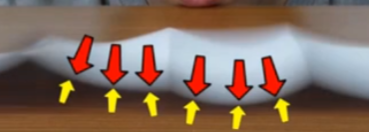
\includegraphics[width=0.45\textwidth]{img/0040.png} 
	\end{tcolorbox}


	
	上面这些现象, 是因为: \textbf{在气体和液体中, 流速越大的位置, 压强越小.} (吹气, 增大了流速).
	
	
	\begin{tcolorbox}[title = {例},boxrule={0.1em},colframe={black!10}, colback={black!3},colbacktitle={black!10},coltitle={black}]
		飞机为什么能够在空中飞行? 原因在于机翼的形状. \\
		
	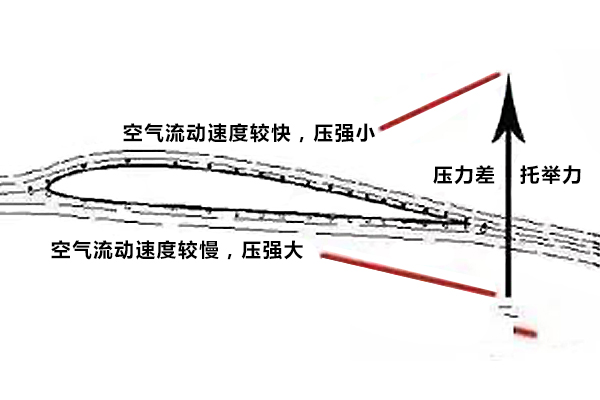
\includegraphics[width=0.45\textwidth]{img/0041.png}
	
	气流被机翼分成上、下两部分, 由于机翼横截面的形状上、下不对称, \textbf{在相同时间内,机翼上方气流通过的路程较长,因而速度较大,它对机翼上表面的压强较小; 而下方气流通过的路程较短,速度较小,它对机翼下表面的压强较大. 这样,机翼上、下表面就存在着压强差,}因而有压力差,这就是产生升力的原因.			
	\end{tcolorbox}



	\begin{tcolorbox}[title = {例},boxrule={0.1em},colframe={black!10}, colback={black!3},colbacktitle={black!10},coltitle={black}]
	火车站, 地铁站的站台上,有一条安全线,人必须站在安全线以外的区域. 否则, 当列车驶过时,人站在安全线以内是非常危险的. 原因就在于列车速度造成的气压差, 会把你推向列车. \\
	
	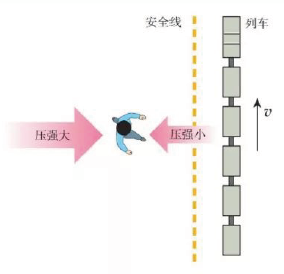
\includegraphics[width=0.45\textwidth]{img/0042.png} 
	\end{tcolorbox}


其他例子还有: 

- 风沿着窗外的墙面吹过时,窗口悬挂的窗帘会飘向窗外. 即室内气压, 大于室外气压. 室内气压把窗帘往外推.


~\\
\hrule
~\\



\section{物体所受的浮力 buoyancy force = 该物体排开的液体或气体的重力G}

物体浸在液体中的体积越大(即物体排开的液体的体积越大)、\textbf{液体的密度越大,则该物体受到的浮力就越大.} \\

阿基米德原理: 大量的实验结果表明, \textbf{浸在液体中的物体受到向上的浮力,浮力的大小, 等于它排开的液体所受的重力.} 即:
\begin{align*}
	\boxed{
	F_{\text{浮力}}=G_{\text{排开的液体或气体的重力}}	
	}
\end{align*}

阿基米德原理, 不仅适用于液体, 也适用于气体.



\begin{tcolorbox}[title = {例},boxrule={0.1em},colframe={black!10}, colback={black!3},colbacktitle={black!10},coltitle={black}]
有一个重7N 的铁球,当它浸没在水中时, 受到多大的浮力? 

根据公式: $F_{\text{浮力}}=G_{\text{排开的液体或气体的重力}}$ \\
我们知道了 $G_{\text{排开的液体或气体的重力}}$, 也就知道了浮力. \\

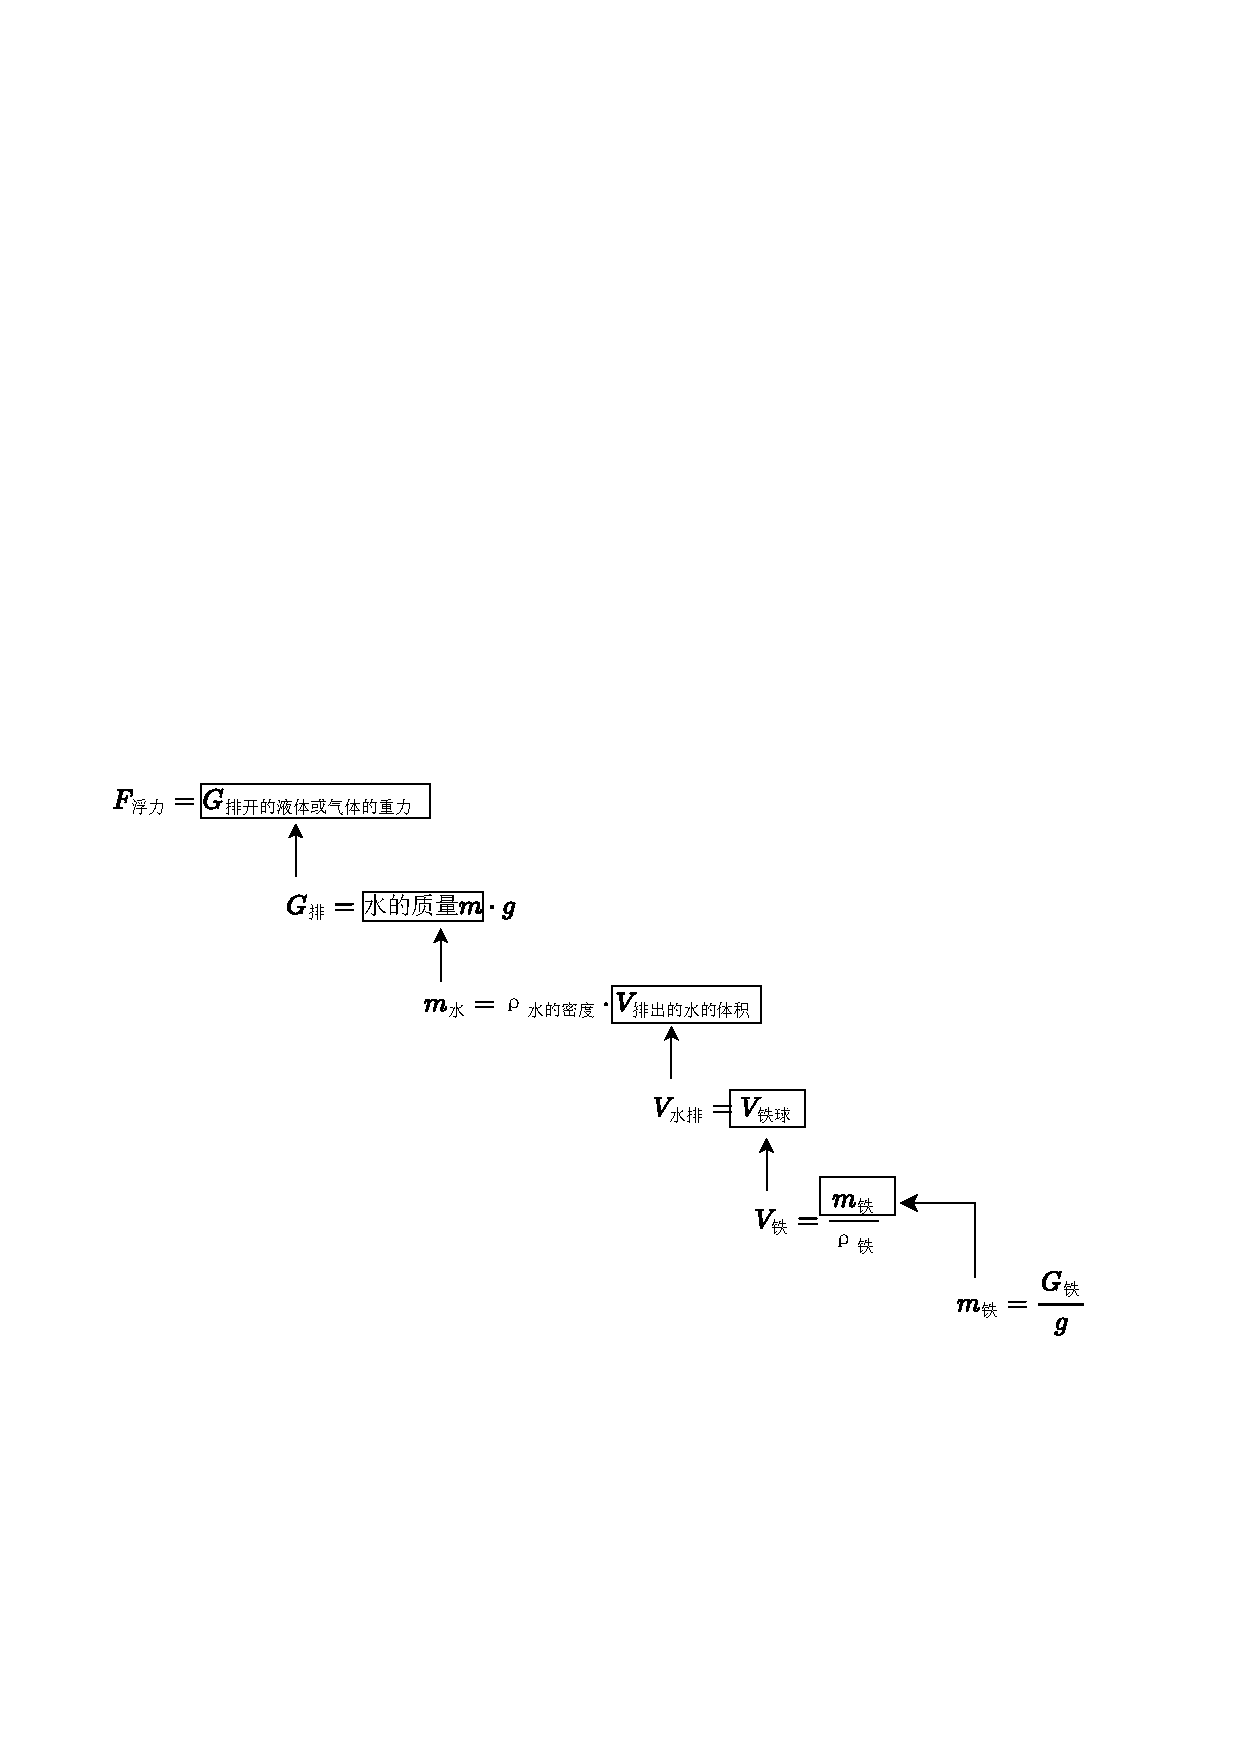
\includegraphics[width=1\textwidth]{img/0043.pdf}

根据上图的公式链, 我们从下往上来一步步求出每一个变量值. 
\begin{align*}
		& (1)\ m_{\text{铁}}=\frac{G_{\text{铁}}}{g}=\frac{7N}{9.8N/kg}=0.714286kg\\
	& (2)\ V_{\text{铁}}=\frac{m_{\text{铁}}}{\rho _{\text{铁的密度}}}=\frac{0.714286\ kg}{7.86\cdot 10^3kg/m^3}=9.08761\times 10^{-5}\ m^3\\
	& \left( 3 \right) \ V_{\text{水排}}=V_{\text{铁}}=9.08761\times 10^{-5}\ m^3\\
	& (4)\ G_{\text{水排}}=m_{\text{水}}g=\rho _{\text{水}}V_{\text{水排}}\cdot g=\left( 1\cdot 10^3kg/m^3 \right) \cdot \left( 9.08761\times 10^{-5}\ m^3 \right) \cdot 9.8N/kg=0.890586N\\
	& \left( 5 \right) \ F_{\text{浮力}}=G_{\text{排开的液体或气体}},\ \text{即}7N\text{重的铁球浮力是}0.89N\\	
\end{align*}

\end{tcolorbox}


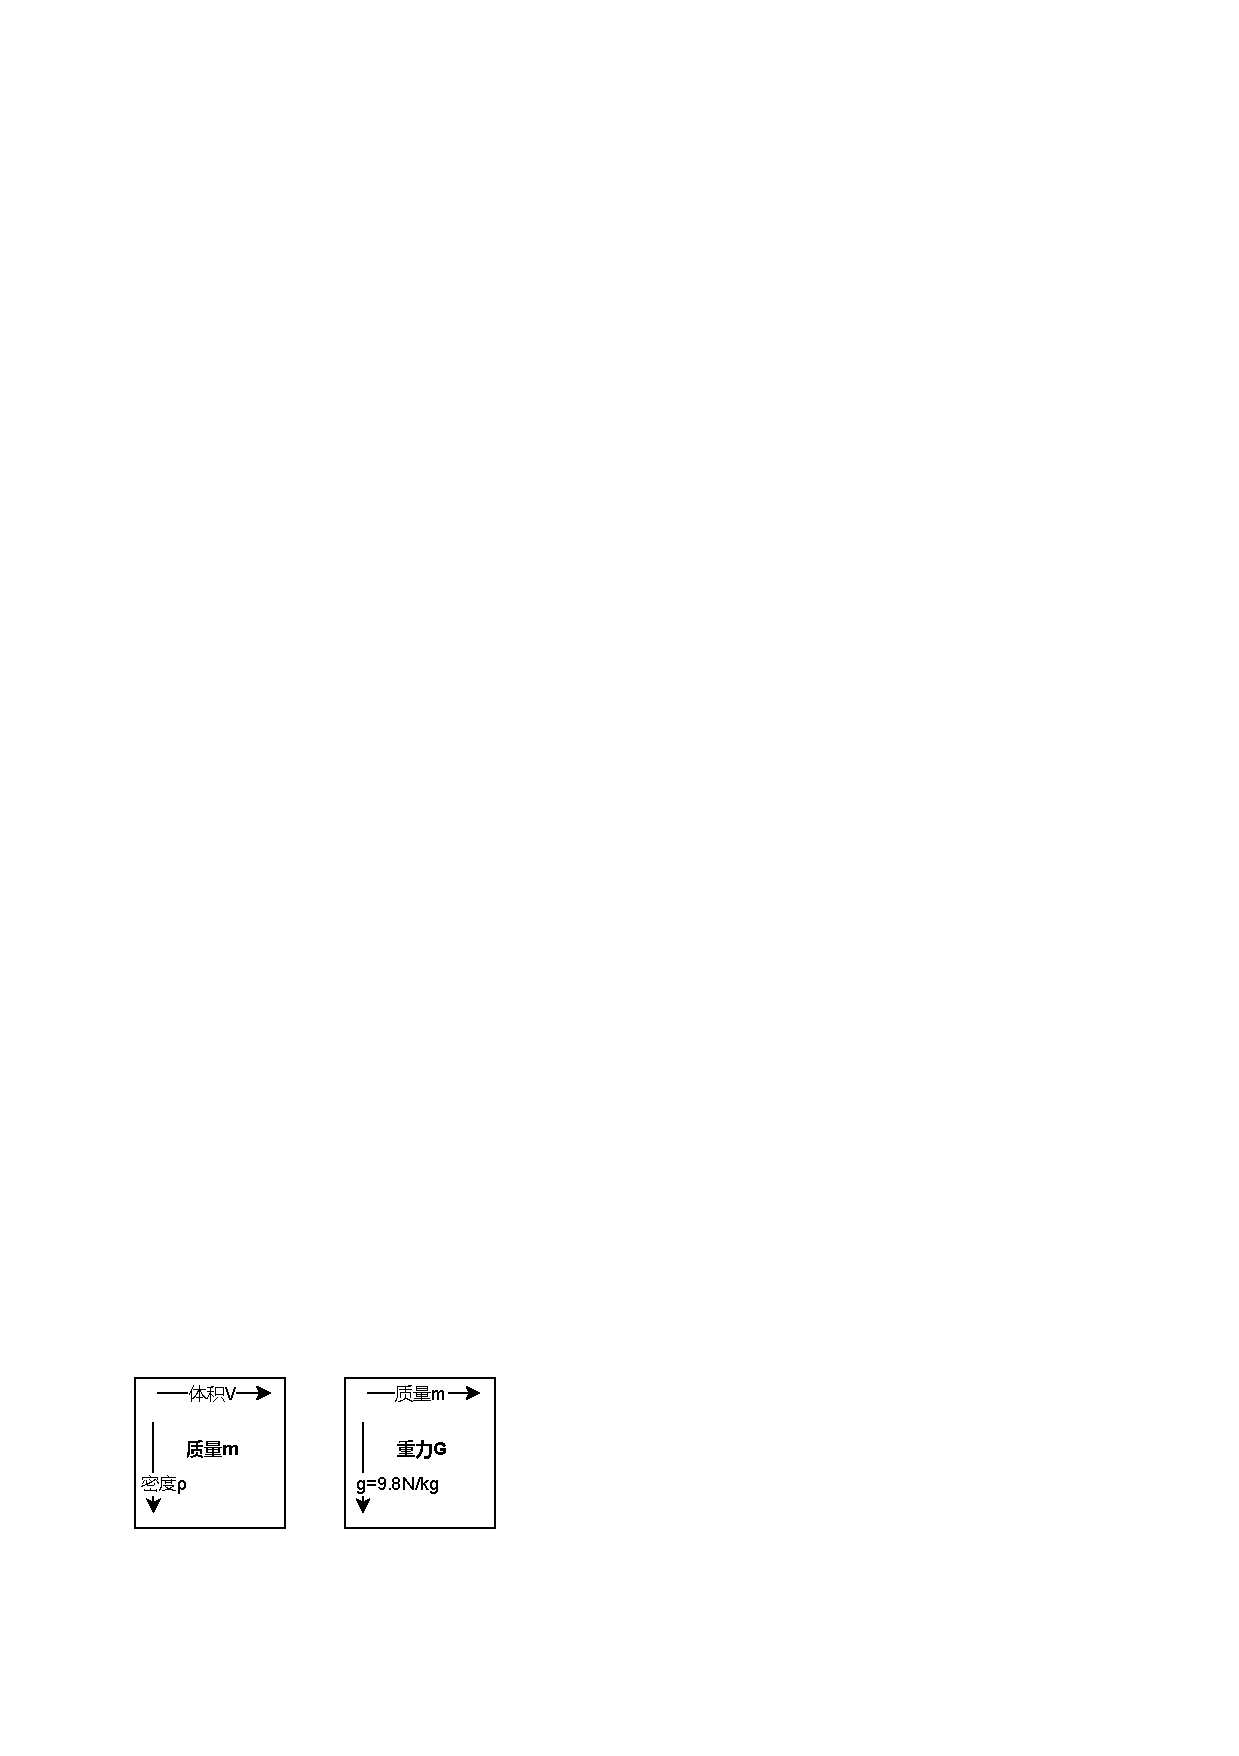
\includegraphics[width=0.4\textwidth]{img/0044.pdf}

浸没在液体中的物体: \\
→ 如果它的密度 < 液体的密度,物体上浮;  \\
→ 如果它的密度 = 液体的密度,物体可以悬浮在液体内任何地方; \\
→ 如果它的密度 > 液体的密度,物体下沉. \\

\begin{tcolorbox}[title = {例},boxrule={0.1em},colframe={black!10}, colback={black!3},colbacktitle={black!10},coltitle={black}]
橡皮泥的密度, 大于水, 所以它在水中会下沉. 但如果把橡皮泥捏成瓢状, 放在水面,\textbf{虽然它的重力G 没有改变,但是排开的水较多, 根据浮力公式}:  	
\begin{align*}
	\boxed{	
	F_{\text{浮力}}=G_{\text{排出的水的重力}}=m_{\text{水}}\cdot g=\left( \rho _{\text{水的密度}}\cdot V_{\text{排出的水的体积}} \right) \cdot g
	}
\end{align*}

\textbf{排开的水的体积变大, 浮力就也同比增加.} 所以橡皮泥船就能漂浮在水面上了. 钢铁轮船能浮在水上, 就是根据这个原理制造的. 
\end{tcolorbox}

轮船的大小, 通常用``排水量"来表示。排水量就是轮船``装满货物"时, 排开水的质量。如一艘轮船,它的排水量是 $1×10^4 t$,就是说此船在满载时,货物质量和船身质量之和, 为$1×10^4 t$.



~\\
\hrule
~\\

\section{功 work = 力F × 移动距离s}

功 work: 如果一个力作用在物体上,物体在这个力的方向上, 移动了一段距离, 就说这个力对物体做了``功".

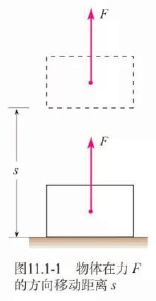
\includegraphics[width=0.2\textwidth]{img/0045.png}

\textbf{力学里所说的做功,包含两个必要因素: (1) 作用在物体上的力, (2) 物体在这个力的方向上移动的距离.}

例如, 如果你搬一块石头而没有搬动, 虽然你对该物体施加了力, 但石头在力的方向上没有移动, 则你对该石头依然没有"做功". \\

力学中,功 = 力 × 物体在力的方向上移动的距离. \\
所以, 作用在物体上的力越大,物体在力的方向上移动的距离越大,力所做的``功"也就越多. \\

公式即:
\begin{align*}
	\boxed{
		\underset{\text{功:单位焦耳}J}{\underbrace{W}}=\underset{\text{力:单位牛}N}{\underbrace{F}}\cdot \underset{\text{沿着力的方向移动的距离,单位:米}}{\underbrace{s}}		
	}
\end{align*}

功的单位, 是牛米. 它有一个专门的名称 -- 焦耳(joule),简称焦, 符号是J. \\



\begin{tcolorbox}[title = {例},boxrule={0.1em},colframe={black!10}, colback={black!3},colbacktitle={black!10},coltitle={black}]
雪橇的质量m=50kg, 上装载木头350kg, 马拉雪橇匀速前进(雪橇受到的摩擦力是800N), 到3km外的目的地. 问马做了多少功? \\
既然马在匀速前行, 说明马的拉力F, 与摩擦力$F_摩$大小相等.

$
\text{功}Work=F_{\text{马的拉力}}\cdot s=F_{\text{雪橇受到的摩擦力}}\cdot s=800N\cdot 3000m=2.4\times 10^6J
$
\end{tcolorbox}
	
	\vspace{1em} 
	
	
	
\subsection{$\text{功率}Power=\frac{\text{功}Work}{\text{时间}time}$ }	

A和B做相同的``功", 完成时间短的, ``做功"快. \\
相同时间内, ``做功"多的那个物体, ``做功"快. \\
	
就像用速度表示运动的快慢一样,在物理学中, \textbf{用``功率"表示做功的快慢. ``功"与``时间"之比, 叫做功率(power).} 公式即:
\begin{align}
	\boxed{
	\underset{\text{功率,单位:瓦特}Watt}{\underbrace{Power}}=\frac{\underset{\text{功,单位:焦耳}}{\underbrace{Work}}}{\underset{\text{时间,单位:秒}}{\underbrace{time}}}		
	}
\end{align}

- 功: 单位是``焦耳" \\
- 时间 : 单位是``秒" \\
- 功率 : 单位是``焦耳每秒",它有个专门的名称叫``瓦特"(watt),简称瓦,符号是W. 功率还有个常用单位是: 千瓦(kW). \\
\begin{align*}
	\boxed{
	1kW = 10^3 W
	}
\end{align*}

\textbf{功率在数值上, 等于单位时间内所做的功.}



\begin{tcolorbox}[title = {例},boxrule={0.1em},colframe={black!10}, colback={black!3},colbacktitle={black!10},coltitle={black}]
	一块石头的质量m=6t, 起重机在15秒内, 将该石头垂直匀速提升了1m, 则该起重器的功率是多少? \\
	
	既然是匀速提升, 则起重机的拉力, 与石头所受的重力相等.	
	\begin{align*}
			&\text{功率}Power=\frac{\text{功}Work}{\text{时间}time}\\
		&=\frac{\text{拉力}F\cdot \text{移动距离}s}{t}=\frac{\overset{=\text{起重机拉力}F}{\overbrace{\text{石头的重力}G}}\cdot s}{t}\\
		&=\frac{\left( m_{\text{石头}}g \right) \cdot s}{t}=\frac{6000kg\cdot 9.8<\frac{N}{kg}>\cdot 1<m>}{15<s>}=3920<Watt>\\		
	\end{align*}
\end{tcolorbox}


	\vspace{1em} 
	

	
	\subsection{动能}
	
	流水, 能推动水车. 子弹, 能击穿靶体. 流水、子弹都做了``功".  \textbf{物体能够对外``做功", 我们就说这个物体具有``能量"(energy),}简称能. \\
	``能量"的单位, 与``功"的单位相同,也是``焦耳".
	
	\textbf{一个物体能够做的``功"越多、表示这个物体的``能量"越大.} \\
	
	运动的钢球打在木块上,木块被推走, 钢球对木块做了功。\textbf{钢球能够做功,表明钢球具有能量。}
	
	\textbf{物体由于运动而具有的能,叫做动能(kinetic energy).} 一切运动的物体都具有动能. \\
	
	kinetic: adj.  /kɪˈnetɪk/  ( technical 术语) of or produced by movement 运动的;运动引起的. kinetic energy 动能 \\
	
	
	动能的大小跟哪些因素有关呢?
	→ 质量m 相同的物体, \textbf{运动的速度越大,它的动能越大} \\
	→ 运动速度相同的物体,\textbf{质量越大,它的动能也越大} \\
	
	
\begin{tcolorbox}[title = {例},boxrule={0.1em},colframe={black!10}, colback={black!3},colbacktitle={black!10},coltitle={black}]
某道路路标显示: 小型客车最高行驶速度不得超过100 km/h. 大型客车、载货汽车最高行驶速度不得超过80 km/h. 限速之差, 正是考虑到动能值的问题.  大车比小车质量大, 如果它们速度相同, 大车的``动能"会大于小车的动能. 因此, 要对不同质量的车型, 限定不同的最高行使速度.
\end{tcolorbox}
	
	\vspace{1em} 
	
	
	\subsection{势能 potential energy}
	
	重力势能: 打桩机, 把重锤高高举起, 重锤落下,可以把桩打入地里,重锤对桩做了功。高处物体所具有的能, 叫做``重力势能". \textbf{物体的质量越大,位置越高,它具有的``重力势能"就越大.	} \\
	
	弹性势能: 拉弯的弓能将箭射出, 具有能量. 这是因为发生形变的物体, 在恢复形变时, 可以做功, 因此具有能量.  \\
	物体由于发生``弹性形变", 而具有的能, 叫做``弹性势能". \textbf{物体的弹性形变越大,它具有的``弹性势能"就越大.}
	
	
	\vspace{1em} 
	
	
	
	\subsection{机械能 = 动能 + 势能}
	
	- 一个物体从高处下落, 物体的``重力势能", 转化成了它的``动能". \\
	- 弯弓射箭时,弓的``弹性势能", 转化成箭的``动能". \\
	- 蹦床运动员从高处落下,在与蹦床面将要接触时,具有一定的动能. 与蹦床面接触后, 床面发生弹性形变, 运动员的``动能", 转化成蹦床的``弹性势能". \\
	可见, \textbf{``动能"和``势能"可以相互转化.} \\
	
	\begin{tcolorbox}[title = {例},boxrule={0.1em},colframe={black!10}, colback={black!3},colbacktitle={black!10},coltitle={black}]
	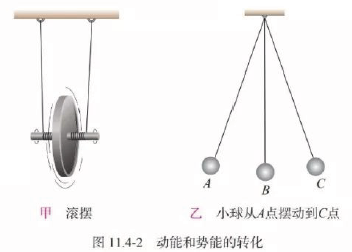
\includegraphics[width=0.4\textwidth]{img/0046.png}
	
	- 上图, 滚摆下降时,它的``重力势能"越来越小,``动能"越来越大,重力势能转化为动能。滚摆上升时,它的``动能"越来越小,``重力势能"越来越大,动能转化为重力势能.
	
	- 上图, \textbf{小球从A点下落到B点,``重力势能"逐渐转化成``动能", 到最低点B时``动能"最大.} 之后又从B点上升到C点, 动能逐渐转化成重力势能.	
	\end{tcolorbox}

	大量研究结果表明,\textbf{如果只有``动能"和``势能"来相互转化的话(即不考虑阻力),尽管动能、势能的大小会变化, 但``机械能"的总和不变. 即: 机械能是``守恒"的.} \\
	
	
	机械能(Mechanical energy), 就是``动能"与``势能"的总和. 这里的``势能", 分为``重力势能"和``弹性势能".  \\
	→ \textbf{决定``动能"的, 是质量, 与速度.} \\
	→ \textbf{决定``重力势能"的, 是质量, 和高度.} \\
	→ \textbf{决定``弹性势能"的, 是劲度系数, 与形变量.} \\
	
	机械能, 是表示物体``运动状态"与``高度"的物理量. \\
	运动状态,是指物体进行``机械运动"时, 相对某个``参考系"的状态。``运动状态"有: 静止、匀速运动、加速运动、减速运动,也有直线运动、曲线运动等多种状态。 \\
	
	
	
	\begin{tcolorbox}[title = {例},boxrule={0.1em},colframe={black!10}, colback={black!3},colbacktitle={black!10},coltitle={black}]
把一个吊起来的铁物, 从你鼻子附近放手, 让它摆来摆去. 想想看,铁物摆回来时, 会打到你的鼻子吗?

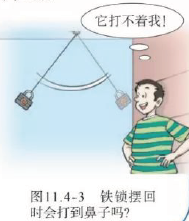
\includegraphics[width=0.25\textwidth]{img/0047.png}
	\end{tcolorbox}
	
	
	
	
	\section{简单机械}






	
	\subsection{杠杆 lever}
	
	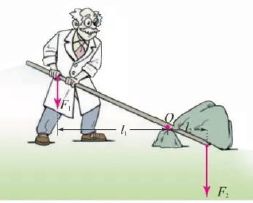
\includegraphics[width=0.4\textwidth]{img/0048.png}
	
	
	杠杆的平衡条件是: 动力×动力臂 = 阻力×阻力臂	
	\begin{align}
		\boxed{
			F_{\text{动力}}\cdot l_{\text{动力臂}}=F_{\text{阻力}}\cdot l_{\text{阻力臂}}			
		}
	\end{align}
	
	
	
	\begin{tcolorbox}[title = {例},boxrule={0.1em},colframe={black!10}, colback={black!3},colbacktitle={black!10},coltitle={black}]
	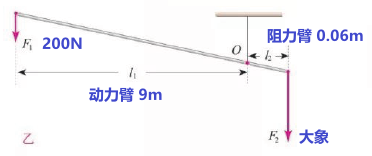
\includegraphics[width=0.4\textwidth]{img/0049.png}	
	\begin{align*}
			& \text{根据公式:\ }\underset{200N}{\underbrace{F_1}}\underset{9m}{\underbrace{l_1}}=\underset{=G_{\text{大象的重力}}}{\underbrace{F_2}}\underset{0.06m}{\underbrace{l_2}}\\
		& F_2=\frac{200\cdot 9}{0.06}=30000N=G_{\text{大象的重力}}=m_{\text{大象的质量}}g\\
		& m_{\text{大象的质量}}=\frac{G_{\text{大象的重力}}}{g}=\frac{30000N}{9.8N/kg}=3061.22kg\approx 3t\\		
	\end{align*}
	\end{tcolorbox}
	
	
	- 等臂杠杆: 动力臂长 = 阻力臂长 \\
	- 省力杠杆: 动力臂长 > 阻力臂长 \\
	- 费力杠杆: 动力臂长 < 阻力臂长 \\
	比如划船, 手移动较小的距离, 使船桨在水中移动较大的距离, 这就是``费力杠杆". 为了省距离, 而费了力气.
	
	
	\vspace{1em} 
	
	
	\subsection{滑轮 pulley}
	
	85
	
	
	\section{内能}
	
	\subsection{分子热运动}
	
	一切物质的分子, 都在不停地做无规则的运动。\textbf{温度越高,分子运动越剧烈.} \\
	由于分子的运动跟温度有关,所以这种无规则运动, 叫做分子的``热运动"(thermal motion). \\
	
	既然分子在运动,那么通常固体和液体中的分子, 为什么不会飞散开,而总是聚合在一起,保持一定的体积呢? 主要是因为\textbf{分子之间存在引力。}分子之间的引力使得固体和液
	体的分子不致散开,因而固体和液体能保持一定的体积。
	
	但物体的分子也不是紧密地挤在一起,而是彼此间存在间隙。为什么压缩固体和液体很困难呢? 这是因为\textbf{除了引力以外, 分子之间还存在斥力。}
	
	
	
	
	
	
	
	
	
	
	
	
	
	
\end{document}